\documentclass[10pt,a4paper]{article}
\usepackage[utf8]{inputenc}
\usepackage[italian]{babel}
\usepackage{amsmath}
\usepackage{amsfonts}
\usepackage{amssymb}
\usepackage{hyperref}		% pacchetto per i link
\usepackage{color}			% pacchetto per colorare il testo
\usepackage{graphicx}		% pacchetto per includere le immagini
\usepackage{svg}				% pacchetto per includere le immagini vettoriali
\usepackage{amsmath}

% rimuove indentazione e aggiunge 3pt di spazio tra i paragrafi
\setlength{\parindent}{0pt}
\setlength{\parskip}{3pt}

\newcommand{\ruolobuono}[1]{{\color{green}{\textbf{#1}}}}
\newcommand{\ruolocattivo}[1]{{\color{red}{\textbf{#1}}}}
\newcommand{\manabuono}{{\color{green}{$\star$}}}
\newcommand{\manacattivo}{{\color{red}{$\star$}}}
\newcommand{\mail}[1]{\href{mailto:#1}{#1}}
\newcommand{\pageurl}[1]{\small\texttt{#1}}
\newcommand{\valpha}{\begin{large}$^\alpha$\end{large}}
\newcommand{\GET}{\texttt{GET}\ }
\newcommand{\lang}[1]{\texttt{#1}}
\newcommand{\PHP}{\lang{PHP}}
\newcommand{\SASS}{\lang{SASS}}
\newcommand{\CSS}{\lang{CSS}}
\newcommand{\pack}[1]{\texttt{#1}}
\newcommand{\NetBeans}{\pack{NetBeans}}
\newcommand{\GameMaster}{$\mathfrak{G\alpha me} \allowbreak \mathfrak{M\alpha ster}$}
\newcommand{\horrule}[1]{\rule{\linewidth}{#1}} 
\newcommand{\lupus}{Lupus in Tabula}
\newcommand{\API}{\texttt{API}}
\newcommand{\gamestatus}[3]{
\textbf{#1}: \textbf{\texttt{#2}}$\quad$ #3
}

\title{
\horrule{0.5pt} \\[0.5cm]
\huge Lupus in Tabula
\horrule{0.5pt}
}

\author{
{\Large Edoardo Morassutto}
}

\date{
{\small Ultimo aggiornamento} \\
\today
}

\begin{document}
\maketitle

Tutto il sorgente è disponibile all'indirizzo: \url{https://github.com/lupus-dev/lupus}

Per contattare l'amministratore: \mail{edoardo.morassutto@gmail.com}

Puoi contattarmi su Facebook se mi hai tra gli amici!

Se vuoi dare una mano ogni tanto forka il repository \texttt{/lupus-dev/lupus} su \texttt{GitHub} e inviaci una \texttt{Pull Request}, se sei stato bravo la mergiamo volentieri!

Se vuoi diventare uno sviluppatore chiedimelo e vedrò di accontentarti!

\section{Introduzione}
Il progetto viene scritto in \PHP. Ovviamente non può mancare l'\lang{HTML}, \lang{CSS}, \lang{JavaScript}, database, git, \lang{SASS}, ed altro\dots

\subsection{Pacchetti software}
Il progetto verrà avviato su una macchina con questi pacchetti (e dipendenze):
\begin{itemize}
\item \pack{Apache2} (qualunque versione recente dovrebbe andare)
	\begin{itemize}
	\item \pack{Mod\_rewrite} (necessaria per il rewrite dell'url)
	\end{itemize}
\item \pack{PHP 5.3} (compatibile con i più comuni webserver gratuiti)
	\begin{itemize}
	\item estensioni varie da definire (le solite comunque)
	\end{itemize}
\item \pack{MySQL} (compatibile con i più comuni webserver gratuiti)
\item \SASS (solo lato compilazione del \CSS)
	\begin{itemize}	
	\item Quindi \pack{Ruby}\dots
	\end{itemize}
\end{itemize}

\subsection{Motivazione delle scelte}
\subsubsection*{Apache2}
Ormai questo è un must dei webserver, nulla da ridire, facile da configurare, veloce, compatibile con tutti i servizi di webhosting gratuiti. 

È necessario abilitare l'estensione \pack{mod\_rewrite} (solitamente è già attiva) per consentire il rewrite degli indirizzi e rendere più accattivante il servizio del gioco.

Tramite il file \texttt{.htaccess} vengono configurate l'estensioni usate, facile il verisioning e la gestione della configurazione.

\subsubsection*{PHP}
Dato che il server del gioco verrà scritto in \PHP, è necessario che \PHP\ sia installato e configurato correttamente. 

Il progetto verrà scritto in \pack{PHP 5.3} (la versione attuale di Altervista) per permettere una facile migrazione di host nel caso sia necessario e per renderlo il più retrocompatibile possibile. Alcune funzioni sono state marcate come \emph{deprecated} in 5.4, sapendolo cerchiamo di evitarle\dots Ad esempio non useremo l'estensione \texttt{mysql} ma la nuova \texttt{mysqli} con approccio ad \emph{oggetti}. È necessario quindi che sia abilitata se non lo fosse già.

\subsubsection*{MySQL}
Per quanto mi possa piacere di più \pack{PostgreSQL} sono costretto a scegliere di usare \pack{MySQL} per le stesse ragioni per cui useremo \pack{PHP 5.3}. \pack{PostgreSQL} non è supportato da Altervista e da altri webhosting gratuiti. 

La versione è abbastanza ininfluente, non useremo funzioni particolarmente recenti.

\subsubsection*{SASS}
\SASS\ è un preprocessore di \CSS, permette di scrivere il \CSS\ molto più semplicemente e di applicare delle particolari formattazioni al file \texttt{.css} in maniera del tutto automatica. Le più importanti differenze tra \CSS\ e \SASS\ sono:
\begin{itemize}
\item In \SASS\ si possono dichiarare le variabili ed effettuare operazioni con esse
\item Si può decidere di comprimere il file \texttt{.css} di output 
\item Si possono annidare le dichiarazioni (vedi manuale del \SASS)
\item È molto più facile da leggere e da mantenere
\item Si possono includere altri fogli \SASS\ dentro un file \SASS\ (aka \emph{import})
\end{itemize}

\SASS\ richiede che sia installato anche \lang{Ruby} per funzionare\dots 

Usando \NetBeans\ è possibile abilitare la compilazione automatica e trasparente dei file \texttt{.scss} ad ogni salvataggio.

\newpage

\section{Il gioco}
\lupus\ è un \emph{gioco di ruolo} molto complesso. Per imparare a giocare si può fare riferimento al nostro amato amico Google\dots

Questa è una semplice guida per iniziare a giocare:

\url{http://www.davincigames.net/lit/lupus_in_tabula_4th_regole.pdf}

Ignorare le carte e pensare in grande per scrivere un server web\dots

\subsection{Struttura dei componenti}
Ovviamente perché si possa chiamare \emph{gioco} è necessario che tutto abbia una struttura solida e chiara. Vengono quindi spiegate le principali entità del gioco. Tutti i riferimenti ai \emph{nomi brevi} sono chiariti nella sezione apposita.

\subsubsection{Gli utenti}
\begin{itemize}
\item Ogni utente che si registra ha un identificativo univoco che fa da chiave primaria
\item Ogni utente ha uno \texttt{username} univoco che usa per identificarsi e per accedere al sito
\item Lo \texttt{username} è un \emph{nome breve}
\item Ogni utente ha un \emph{livello} pubblico che determina i privilegi a cui l'utente può accedere
\item Ogni utente ha una email che viene usata per verificare l'account e notificare qualcosa\dots \emph{(da definire)}
\end{itemize}

\subsubsection{Le stanze}
\begin{itemize}
\item Ogni utente può creare un certo numero di stanze (in base al livello)
\item Ogni stanza può contenere più partite, una sola però può essere attiva
\item Ogni stanza ha un nome breve \texttt{room\_name}
\item Ogni stanza ha una descrizione con lo stesso grado di accessibilità della stanza
\item Le stanze possono essere private o pubbliche
\item Ogni utente può visualizzare una stanza pubblica
\item Solo gli utenti partecipanti e/o autorizzati possono visualizzare una stanza privata
\item Ogni stanza ha un amministratore, colui che ha creato la stanza
\item Le stanze possono essere eliminate
\end{itemize}

\subsubsection{Le partite}
\begin{itemize}
\item Ogni partita è interna ad una stanza
\item Ogni partita ha un nome breve unico per quella stanza (\texttt{game\_name})
\item Ogni partita ha una descrizione scelta dall'amministratore della stanza
\item L'amministratore della partita è l'amministratore della stanza corrispondente
\item Possono essere create delle partite solo se non ci sono partite attive
\item Gli utenti possono essere invitati nella partita oppure possono richiedere all'amministratore di farne parte
\item La partita può iniziare solo se è presente il numero di giocatori richiesto
\item La partita viene avviata dall'amministratore
\item L'amministratore può espellere un giocatore
\item L'amministratore può terminare la partita
\item I ruoli dei giocatori vengono rilevati solo al termine della partita
\item La chat della partita rimane visibile solo ai giocatori
\item Eventuali altre chat vengono disabilitate alla fine della partita
\end{itemize}

\subsubsection{I livelli}
\begin{itemize}
\item Ogni utente ha un livello
\item Il livello è solo crescente (non si può essere degradati tranne dal \GameMaster)
\item Un utente bannato ha livello uguale a \emph{zero} (da definire\dots)
\end{itemize}

\subsubsection{Nomi brevi}
Tutti i riferimenti ai nomi brevi sono da intendere che rispettano le seguenti caratteristiche:
\begin{itemize}
\item Hanno una lunghezza di al più 10 caratteri
\item Hanno una lunghezza di almeno un carattere
\item Sono formati da soli caratteri ASCII alfanumerici
\item Il primo carattere è una lettera
\item Ogni nome breve è unico rispetto al proprio contesto
\end{itemize}


\subsection{Struttura del server}

\subsubsection*{Modulare}
Il \emph{server} e le \API\ sono gestite nel modo più modulare possibile:

Deve essere possibile avere una cartella dove mettere dei file \PHP\ contenenti i ruoli. Aggiungere e togliere dei ruoli deve essere una semplice modifica del relativo file in questa cartella. 

Non deve essere presente un file dove vengono registrati i ruoli, deve essere gestito in maniera automatica e dinamica.

\subsubsection*{Orientato agli oggetti}
Ogni ruolo deve essere un oggetto che deriva dalla classe \texttt{Role}.

I file \PHP\ contenenti le informazioni di un ruolo devo chiamarsi \texttt{role.\textit{Ruolo}.php} dove ruolo è il nome della classe e del ruolo con l'iniziale \emph{maiuscola}.

Il nome del ruolo è un nome breve.

Se un giocatore ha un ruolo non esistente o non abilitato la partita termina a causa di un errore interno.

\subsection{Ruoli}
I ruoli da implementare fin da subito potrebbero essere: (il colore indica la fazione, la stella il mana)
\begin{itemize}
\item \ruolocattivo{Lupo\manacattivo} Durante la notte i \emph{lupi} votano chi eliminare, se almeno il 50\%+1 dei \emph{lupi} vivi votano la stessa persona, questa è una candidata a morire;
\item \ruolobuono{Guardia\manabuono} Durante la notte la \emph{guardia} può scegliere di proteggere una persona, se i \emph{lupi} quella notte decidessero di ucciderla, essa non muore;
\item \ruolobuono{Medium\manabuono} Il \emph{medium} durante la notte può scegliere di guardare un giocatore morto, lui saprà se quel giocatore aveva un mana buono o cattivo;
\item \ruolobuono{Veggente\manabuono} Il \emph{veggente} può fare le stesse operazioni del \emph{medium}, solo sui giocatori vivi;
\item \ruolobuono{Paparazzo\manabuono} Il \emph{paparazzo} durante la notte sceglie una persona da pedinare, vengono riportati sul giornale della mattina seguente tutti i giocatori che hanno visitato il personaggio \textsl{paparazzato};
\item \ruolobuono{Criceto mannaro\manacattivo} \'E un giocatore normale, senza poteri speciali. Se la partita termina e lui è ancora vivo allora vince solo lui e non la sua fazione;
\item \ruolobuono{Assassino\manacattivo} L'\emph{assassino} una sola volta nella partita può scegliere una persona e ucciderla;
\item \ruolobuono{Massone\manabuono} I \emph{massoni} non hanno poteri però hanno una chat dedicata e quindi si conoscono tra loro;
\item \ruolobuono{Contadino\manabuono} I \emph{contadini} non hanno poteri\dots
\item \ruolobuono{Pastore\manabuono} I \emph{pastori} possono scegliere di sacrificare delle pecore per salvare dei giocatori dalle grinfie dei lupi;
\item \ruolobuono{Falso\manacattivo} Il \emph{falso} può scegliere tra una serie di proposizioni false e renderle pubbliche sul giornale;
\item \ruolobuono{Prescelto\manabuono} Il \emph{prescelto} all'inizio della partita conosce 4 proposizioni, 2 vere e 2 valse;
\item \ruolobuono{Sindaco\manabuono} Il \emph{sindaco} è un contadino che non può essere messo al rogo nella votazione diurna;
\end{itemize}

\subsection{Stati partita}
Ogni partita contiene il campo \emph{status}, un valore intero che rappresenta lo stato di gioco della partita.

Lo stato della partita divide ogni partita in 3 fasi:

\subsubsection{Fase pre-partita}
Questa fase è presente solo prima dell'avvio della partita e serve per salvare ed aggiustare i dettagli della partita, come il numero di giocatori, di ruoli, la descrizione, ecc\dots

Questa fase è identificata da codici nell'intervallo:
\[
	0 \le x < 100
\]

I codici riconosciuti sono:
\begin{itemize}
\item \gamestatus{0}{Setup}{Impostazione della partita}
\end{itemize}

\subsubsection{Fase in-partita}
Questa fase è presente poco prima dell'inizio della partita e durante tutto il corso della partita. 

Viene identificata da codici nell'intervallo:
\[
	100 \le x < 200
\]

I codici riconosciuti sono:
\begin{itemize}
\item \gamestatus{100}{NotStarted}{La partita è attiva e i giocatori possono iniziare ad entrare}
\item \gamestatus{101}{Started}{La partita è in corso e i giocatori non possono più entrare}
\end{itemize}

\subsubsection{Fase terminata in modo corretto}
Questa fase si verifica quando la partita termina in modo corretto e viene scelta una squadra vincitrice.

I codici che la identificano sono compresi nell'intervallo:
\[
	200 \le x < 300
\]

I codici riconosciuti sono:
\begin{itemize}
\item \gamestatus{200\,+\,y}{Win$y$}{La partita è terminata e ha vinto la squadra $y\ (0\le y < 99)$}
\item \gamestatus{299}{DeadWin}{La partita è terminata perché tutti i giocatori sono morti}
\end{itemize}

\subsubsection{Fase terminata in modo inaspettato}
Questa fase si verifica quando la partita viene interrotta prima della sua normale fine. In questo caso non viene designato alcun vincitore.

I codici che identificano questa fase sono compresi dall'intervallo:
\[
	300 \le x < 400
\]

I codici riconosciuti sono:
\begin{itemize}
\item \gamestatus{300}{TermByAdmin}{L'amministratore della stanza ha fatto terminare la partita}
\item \gamestatus{301}{TermBySolitude}{Un numero eccessivo di giocatori hanno abbandonato la partita}
\item \gamestatus{302}{TermByVote}{\'E stato raggiunto il \emph{quorum} per terminare la partita}
\item \gamestatus{303}{TermByBug}{Un errore interno del server ha fatto terminare la partita per preservare l'integrità del server}
\item \gamestatus{304}{TermByGameMaster}{Il \GameMaster\ ha deciso di terminare la partita}
\end{itemize}

\subsection{Misura del tempo}
Il tempo in \lupus\ si suddivide in tre \emph{tipi}:
\begin{itemize}
\item Arrivo al villaggio
\item Giorno
\item Notte
\end{itemize}

Il passare del tempo viene memorizzato nel campo \texttt{day} di una partita e il suo \emph{tipo} viene distinto usando la seguente formula:

\[
	day
	\left\{
	\begin{aligned}
	\text{se}\ day = 0 						&\Rightarrow \text{arrivo al villaggio} \\
	\text{se}\ day\ \text{è \emph{pari}}		&\Rightarrow \text{giorno}\ \frac{day}{2}+1 \\
	\text{se}\ day\ \text{è \emph{dispari}}	&\Rightarrow \text{notte}\ \frac{day}{2}+1
	\end{aligned}
	\right.
\]

\section{Il server}
Il server è suddiviso in più parti:
\begin{itemize}
\item Il \emph{database}
\item Le \API
\item La \emph{web-app}
\end{itemize}

\subsection{Il database}
Il \emph{database} è formato da una serie di tabelle spiegate nel dettaglio nella sezione dedicata più avanti.

\subsection{Le API}
A causa della natura dinamica del gioco sono necessarie delle funzioni accessibili facilmente tramite \lang{JavaScript}. Tramite queste funzioni è possibile far proseguire la partita, ottenere informazioni ed effettuare richieste al server.

\subsubsection*{Funzioni disponibili}
Tutte le seguenti funzioni si intendono già nel percorso delle \API\ (es: \pageurl{/api}). 

\valpha~indica che la funzione non è completa.

\begin{itemize}
\item \pageurl{/login} Effettua il login tramite \texttt{username/password} e salva nella \emph{sessione} l'identificativo dell'utente. Devono essere specificati i parametri \texttt{username} e \texttt{password} tramite \GET

\item \pageurl{/login/(username)} Sostituisce il metodo precedente. Effettua il login dell'utente specificato. La password va specificata in \GET come per \pageurl{/login}. Se viene specificato anche lo \texttt{username} in \GET viene ignorato.

\item \pageurl{/logout} Se l'utente è connesso lo disconnette cancellando la sessione

\item \pageurl{/status\valpha} Mostra delle informazioni sul server, come la versione, ecc..

\item \pageurl{/user/(username)} Mostra le informazioni dell'utente specificato

\item \pageurl{/me} Scorciatoia per \pageurl{/user/(username)} con lo \texttt{username} dell'utente 

\item \pageurl{/room/(room\_name)} Mostra le informazioni della stanza specificata

\item \pageurl{/game/(room\_name)/(game\_name)} Mostra le informazioni della partita specificata

\item \pageurl{/new\_room/(room\_name)} Crea una nuova stanza appartenente all'utente. Deve venire specificato il parametro \texttt{descr} in \GET. Può essere specificato il parametro \texttt{private} per rendere la stanza privata

\item \pageurl{/new\_game/(room\_name)/(game\_name)} Crea una nuova partita nella stanza specificata. Devono venire specificati i parametri \texttt{descr} e \texttt{roles} in \GET
\end{itemize}

\subsection{La web-app}
L'interfaccia grafica del gioco sarà sviluppata con la libreria \texttt{BootStrap}, la quale rende tutto molto portabile su dispositivi con schermo ridotto. 

Non ci sarà troppo \PHP\ in queste pagine, il grosso del lavoro sarà il \lang{JavaScript} a farlo, in coppia con le \API.

\subsubsection*{Pagine}
Quello che segue è un elenco delle pagine che devono essere implementate
\begin{itemize}
\item \pageurl{/index} è la pagina che contiene i link alle varie pagine del gioco. Accessibile solo dopo il \emph{login}.
\item \pageurl{/login} è la pagina per accedere al sito
\item \pageurl{/admin} è una pagina che contiene la lista dei collegamenti alle altre pagine di amministrazione 
\item \pageurl{/admin/(room\_name)} è la pagina di amministrazione di una stanza
\item \pageurl{/admin/(room\_name)/(game\_name)} è la pagina di amministrazione di una partita
\item \pageurl{/game} è una pagina che contiene la lista dei collegamenti alle altre pagine di gioco
\item \pageurl{/game/(room\_name)} è una pagina che contiene le partite di una stanza
\item \pageurl{/game/(room\_name)/(game\_name)} è la pagina di gioco di una partita
\item \pageurl{/user} è la pagina dell'utente
\item \pageurl{/user/(username)} è la pagina di un utente specifico
\item \pageurl{/status} contiene lo stato del server (numero di partite, di stanze, ecc\dots)
\item \pageurl{/join} è la pagina per trovare una partita
\item \pageurl{/singup} è la pagina per registrarsi
\end{itemize}

\newpage

\section{Il database}
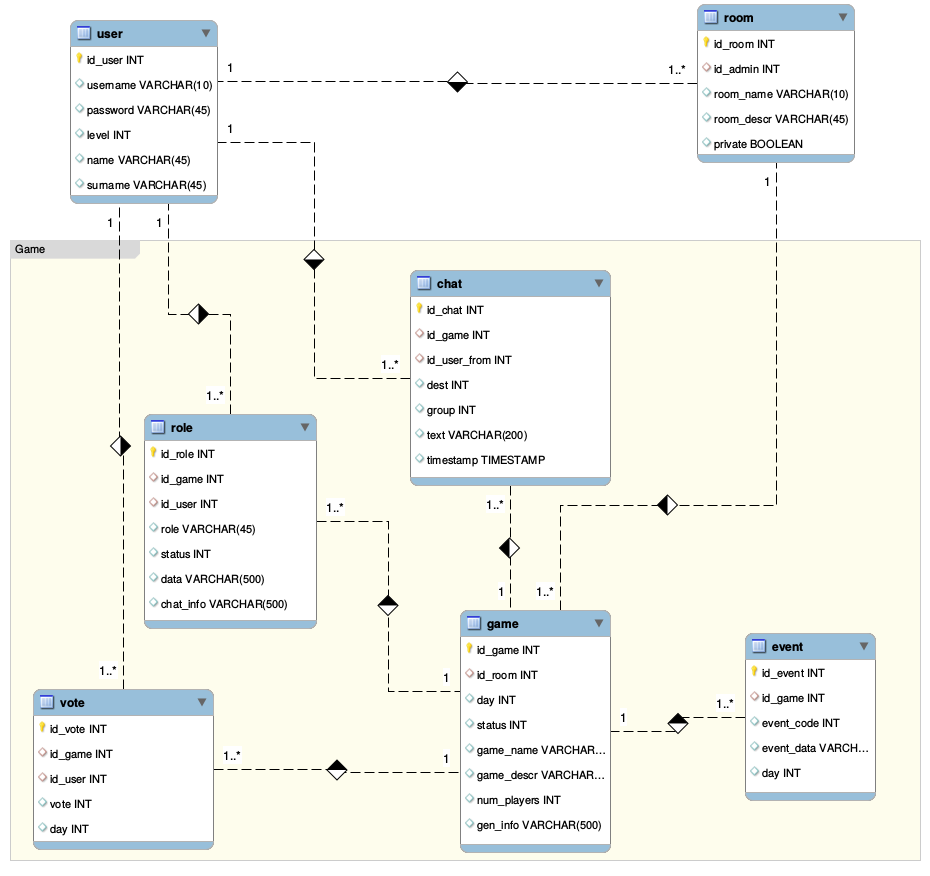
\includegraphics[width = \textwidth]{database.png}

Questa è una \emph{bozza} della struttura del database, ci saranno sicuramente molte modifiche. Lo schema \texttt{E-R} è stato disegnato con il programma \texttt{MySQL Workbench}.

\subsection{Tabella user}
In questa tabella vengono memorizzati gli utenti registrati. Ogni utente ha un \texttt{id\_user} che rimane nascosto al pubblico e identifica all'interno del database uno ed un solo utente. Ogni utente è identificato all'esterno con un \texttt{username} unico che rispetta il formato \emph{nome breve}.

La password dell'utente è salvata codificata in \texttt{SHA-1}. In futuro potrebbe essere aggiunto un ulteriore livello di protezione aggiungendo del \emph{salt}.

Il livello dell'utente è salvato nella righe dell'utente. Ogni volta che si verifica un evento che potrebbe modificare il livello, si ricalcola il livello e lo si aggiorna solo se è strettamente maggiore di quello precedente.

Ogni utente ha anche un campo \texttt{name} e uno campo \texttt{surname}

\subsection{Tabella room}
La tabella \texttt{room} contiene le informazioni delle stanze. 

Ogni stanza ha un identificativo univoco \texttt{id\_room}, nascosto al pubblico che identifica la stanza all'interno del database. 

Ogni stanza contiene l'identificativo dell'utente amministratore della stanza \texttt{id\_admin}. 

Al pubblico la stanza è identificata con un nome \texttt{room\_name} il quale è unico. Ogni stanza ha anche una descrizione \texttt{room\_descr} che rappresenta il titolo della stanza. 

Il campo \texttt{private} indica se la stanza è privata.

\subsection{Tabella game}
La tabella game raccoglie le informazioni di ogni partita. 

Ogni partita è identificata all'interno del database con un identificativo unico \texttt{id\_game}. 

Ogni partita è contenuta all'interno di una stanza \texttt{id\_room}. 

Ogni partita è identificata all'esterno con un \emph{nome breve} unico all'interno della stessa stanza \texttt{game\_name}, inoltre ogni partita ha una descrizione che rappresenta il titolo della partita \texttt{game\_descr}.

I campi \texttt{day} e \texttt{status} sono informazioni utili della partita, l'istante temporale del gioco e lo stato della partita.

Il campo \texttt{roles} contiene una stringa \texttt{JSON} che codifica un vettore associativo con il numero di personaggi di ogni ruolo presente nella partita.

\subsection{Tabella role}
In questa tabella sono memorizzati i ruoli dei giocatori interni ad una partita. 

Ogni riga è identificata da un campo \texttt{id\_role} non pubblico. 

Ogni ruolo è interno alla partita \texttt{id\_game} e relativo all'utente \texttt{id\_user}. 

Il ruolo dell'utente è memorizzato nella stringa \texttt{role} la quale identifica un ruolo nella cartella dei ruoli. 

Il campo \texttt{status} indica lo stato dell'utente (vivo o morto). 

Alcuni ruoli potrebbero richiedere di memorizzare delle informazioni aggiuntive, il campo \texttt{data} contiene dei dati salvati da un ruolo, codificati in \texttt{JSON}.

\subsection{Tabella vote}
In questa tabella vengono memorizzati i voti degli utenti. 

Ogni voto è identificato tramite il campo \texttt{id\_vote}, il quale rimane nascosto all'esterno del database. 

Ogni voto è specifico della partita \texttt{id\_game} nel momento \texttt{day} e appartiene all'utente \texttt{id\_user}. 

Il suo voto è \texttt{vote} il quale può essere l'identificativo di un utente, un voto \emph{nullo} o altro. 

\subsection{Tabella chat}
In questa tabella vengono memorizzati i messaggi delle varie chat. 

Ogni messaggio è identificato all'interno del database da \texttt{id\_chat}. 

Ogni messaggio si riferisce alla partita \texttt{id\_game}. 

Il mettente del messaggio è \texttt{id\_user\_from} cioè l'identificativo dell'utente che ha inviato il messaggio. 

Il destinatario \texttt{dest} è un numero intero che può rappresentare vari identificativi, in base a \texttt{level} il destinatario può essere un utente, il pubblico, una chat privata, ecc\dots

Il testo del messaggio è \texttt{text} il quale non può essere più lungo di 200 caratteri e viene eseguito l'\emph{escape} sia per il database che per il \lang{JavaScript}.

\subsection{Tabella newspaper}
In questa tabella viene memorizzato il giornale dei vari giorni della partita. 

Ogni articolo è identificato da \texttt{id\_news} ed appartiene alla partita \texttt{id\_game} al tempo \texttt{day}. 

Il testo dell'articolo è memorizzato in \texttt{news}.

\newpage
\tableofcontents

\end{document}